\section{Teoría de juegos}

La teoría de juegos es una herramienta fundamental para entender las estrategias en interacciones de todo tipo en la economía. Modelar sirve para entender los elementos que entran en juego los cuales se pueden instrumentalizar con tal de obtener una situación deseado, como puede ser incentivar la cooperación o la competencia en un mercado. 

Esta rama es fundamentalmente matemática, puede ser tan simple como compleja. En este capítulo se tratará lo más básico de teoría de juegos simultáneos, secuenciales, iterados y demás. 

La sustancia de un juego se compone de tres elementos: jugadores, estrategias y pagos. Los jugadores son quienes toman decisiones de manera estratégica para maximizar el pago posible que obtengan al final de un juego. El componente estratégico surge del hecho de que las decisiones de otros influyen los pagos que obtenga un jugador dada la decisión que tomó. En la economía hay multitud de estas interacciones, por ejemplo el precio fijado por una empresa afecta la demanda del bien de su competencia. 

Para introducirnos en la materia empezaron dando ejemplos (no necesariamente económicos) para definir juegos simultáneos.

\subsection{Juegos simultáneos}

En juegos simultáneos los jugadores toman decisiones al mismo tiempo, estas decisiones interactuan resultando en pagos. El pago a cada persona refleja un nivel de utilidad, por lo que cada agente buscará llegar a un resultado del juego (la combinación de acciones) que maximize su pago. 

Para dos agentes $A$ y $B$ cada uno toma la decisión $X$ o $Y$, la combinación de decisiones llevará a cierto nivel de pagos. Este escenario puede ser representado por una \textbf{matriz de pago}\marginnote{\textbf{Matriz de pago:} La matriz de pago es la representación de los pagos un juego dados ciertos jugaroes y estrategias posibles.}[-3cm] en el cuadro \ref{cuadro: matriz de pago genérica}.

\begin{table}[!htbp]
  
  \centering
  \caption{Matriz de pagos}
  \setlength{\extrarowheight}{2pt}
  \label{cuadro: matriz de pago genérica}
  \begin{tabular}{*{4}{c|}}
    \multicolumn{2}{c}{} & \multicolumn{2}{c}{$B$}\\\cline{3-4}
    \multicolumn{1}{c}{} &  & X  & Y \\\cline{2-4}
    \multirow{2}*{$A$}  & X & $(a,b)$ & $(c,d)$ \\\cline{2-4}
    & Y & $(e,f)$ & $(g,h)$ \\\cline{2-4} 
  \end{tabular}
\end{table}

La tabla nos dice que si $A$ tomó la estrategia $X$ y $B$ toma la decisión $Y$ entonces los pagos correspondientes son $(c,d)$, donde $c$ es el pago para $A$ y $d$ el pago para $B$. De la misma manera si $A$ elije $Y$ y $B$ decide $Y$ la matriz de pagos será $(g,h)$. 

La matriz también representa el componente estratégico mencionado en un inicio. Los pagos posibles para $A$ claramente dependen de las decisiones que tome $B$. Para poder decidir de manera estratégica los jugadores miran al futuro, si $A$ sabe que $B$ decide $X$ entonces $A$ elegirá la estrategia que maximize sus pagos. Específicamente $A$ está decidiendo con respecto a los pagos en negrita en el cuadro \ref{cuadro: B decide X}.

\begin{table}[!htbp]
  \centering
  \caption{Matriz de pagos con $B$ decidiendo $X$} \label{cuadro: B decide X}
  \setlength{\extrarowheight}{2pt}
  \begin{tabular}{*{4}{c|}}
    \multicolumn{2}{c}{} & \multicolumn{2}{c}{$B$}\\\cline{3-4}
    \multicolumn{1}{c}{} &  & X  & Y \\\cline{2-4}
    \multirow{2}*{$A$}  & X & $(\textbf{a,b})$ & $(c,d)$ \\\cline{2-4}
    & Y & $(\textbf{e,f})$ & $(g,h)$ \\\cline{2-4}  
  \end{tabular}
\end{table}

La decisión que tome $A$ dependerá qué pago es mayor, $a$ ó $e$, si es $a$ entonces elije $X$ y caso contrario elije $Y$.

Ahora veremos diversos juegos canónicos con el objetivo de aprender a resolver estos juegos y dar un análisis bajo criterio de Pareto de los mismos.

\subsection{El Dilema del Prisionero, un Juego Canónico}

El dilema del prisionero describe la situación en que dos criminales sospechosos son detenidos y separados para un proceso de interrogación. Si uno de los dos delata al otro y su complice no, este último tendrá pena de cárcel y el delator quedará libre. En caso de que los dos se delaten entre sí, ambos son condenados a años de cárcel. Por útlimo si ninguna se delata entre sí, quedan libres o cumplen penas menores.

La situación se ve reflejada en la matriz de pago del cuadro \ref{Juego: Prisionero}. Vemos que a mayor pena menores son los pagos. La solución de este juego es la siguiente.

\begin{table}[!htbp]
    \centering
    \caption{El dilema del prisionero}
    \setlength{\extrarowheight}{2pt}
    \begin{tabular}{*{4}{c|}}
      \multicolumn{2}{c}{} & \multicolumn{2}{c}{Prisionero $B$}\\\cline{3-4}
      \multicolumn{1}{c}{} &  & Cooperar  & Delatar \\\cline{2-4}
      \multirow{2}*{Prisionero $A$}  & Cooperar & $(-2,-2)$ & $(-10,-1)$ \\\cline{2-4}
      & Delatar & $(-1,-10)$ & $(-6,-6)$ \\\cline{2-4}
    \end{tabular} \label{Juego: Prisionero}
  \end{table}

Los jugadores deciden su estrategia óptima mirando hacia el futuro y prediciendo si es posible la decisión del otro. Si el prisionero $A$ piensa que $B$ lo delatará su respuesta óptima sería delatarlo también, dado que es la opción que minimiza sus años de cárcel. En caso de que $B$ coopere la respuesta óptima de $A$ sería delatar igualmente, dado que sigue siendo la opción que minimiza sus años de cárcel. Notemos que $A$ sigue la estrategia delatar independiente de la decisión de $B$, a esto se le llama una \textbf{estrategia dominante}\marginnote{\textbf{Estrategia Dominante:} }[0cm].

La matriz de pago es simétrica para ambos jugadores entonces llegamos a que $B$ sigue el mismo razonamiento por lo que delatar será también su estrategia dominante.

Dado que ambos tienen un estrategia dominante por delatar el resultado del juego será (Delatar, Delatar), dando un matríz de pago ($-6,-6$). Este punto se le conoce como \textbf{equilibrio de Nash}\marginnote{\textbf{Equilibrio de Nash:} }[0cm], es un punto tal que dada las decisiones tomadas por los demás jugadores ningun jugador tendrá incentivo a cambiar de decisión. Lo cual es equivalente a que cada uno eligió su estrategia óptima frente a las decisiones de los demás. En este caso sería que, dado que $B$ delató, $A$ no tiene incentivos a cambiar su decisión a cooperar, lo mismo se puede decir de $B$.

Hasta ahora hemos descrito un juego, es decir, jugadores, estrategias y pagos. Se resolvió este juego en específico donde dado que ambos jugadores tenían una estrategia dominante por delatar se llegó a un equilibrio de Nash. El siguiente paso es comentar sobre distintos aspectos del resultado bajo el criterio de Pareto.

El resultado fue (Delatar, Delatar) sin embargo otra posibilidad es que los jugadores hayan cooperado (Cooperar, Cooperar), en cuyo caso ambos jugadores están mejor. Esto bajo el criterio de Pareto se le llamaría una mejoría de pareto: si es que ambos cooperaran todos estarían mejor. Bajo esta perspectiva podemos decir que el equilibrio encontrado en este juego es sub-óptimo en términos de Pareto dado que hay un resultado posible mejor para ambos.

Este resultado es crucial pues es aplicable a un diversas situaciones económicas y políticas típicas, donde la cooperación nos llevaría a mejores resultados pero dada la desconfianza llegamos a un equilibrio sub óptimo. Por ejemplo, dos países con armas nucleares pueden acordar desarmarse para aumentar la seguridad mutua. Si ambos cumplen el acuerdo (cooperan), ambos estarán seguros y reducirán costos militares. Si uno cumple y el otro no (no coopera), el que deserta obtiene ventaja militar. Si ambos desertan y no desarman, continúan con altos costos y riesgos de conflicto. 

La gran moraleja económica en este caso es que dejar que los agentes decidan bajo sus propios intereses no siempre lleva al mejor resultado posible, la intervención en estos casos puede ser justificable. Ahora veremos otros juegos canónicos para describir otro tipo de situaciones.

\subsection{Otros Juegos Canónicos}

\textsc{Mano Invisible}

La matriz que representa este juego se encuentra en el cuadro \ref{Juegos: Mano}. La mano invisible describe cómo los individuos que buscan su propio beneficio personal, sin intención de hacerlo, contribuyen al bienestar general de la sociedad. Si se deja la autorregulación de los mercados, dado que los individuos persiguen su propio interés, se produce un equilibrio óptimo de Pareto. El agente $A$ tendrá una estrategía dominante la cual será la opuesta que el jugador $B$. Finalmente el equilibrio de Nash es eficiente paretianamente.

\begin{table}[!htbp]
    \centering
    \caption{La mano invisible}
    \setlength{\extrarowheight}{2pt}
    \begin{tabular}{*{4}{c|}}
      \multicolumn{2}{c}{} & \multicolumn{2}{c}{Agente $B$}\\\cline{3-4}
      \multicolumn{1}{c}{} &  & $X$  & $Y$ \\\cline{2-4}
      \multirow{2}*{Agente $A$}  & $X$ & $(0,10)$ & $(1,1)$ \\\cline{2-4}
      & $Y$ & $(11,11)$ & $(10,0)$ \\\cline{2-4}
    \end{tabular} \label{Juegos: Mano}
  \end{table}

%(Aquí se podría citar a Adam Smith)

\textsc{Guerra de los sexos}

Este juego se puede representar con la matriz del cuadro \ref{Juegos: Guerra}. La historia detras refiere a una pareja que se encuentra incomunicada en medio de un festival de música. Ambos tienen gustos diferentes, al hombre le gusta el Reggae mientras que a la mujer le gusta el EDM. Dado que están separados e incomunicados quieren encontrarse, pero también quieren ir al concierto que sea la música de su gusto. Es por eso que reciben utilidad tanto de encontrarse como de ir al concierto que les gusta, maximizan su utilidad si es que van al concierto de su preferencia y encuentran a su pareja ahí.
\begin{table}[!htbp]
    \centering
    \caption{Guerra de los sexos}
    \setlength{\extrarowheight}{2pt}
    \begin{tabular}{*{4}{c|}}
      \multicolumn{2}{c}{} & \multicolumn{2}{c}{Mujer}\\\cline{3-4}
      \multicolumn{1}{c}{} &  & Reggae  & EDM \\\cline{2-4}
      \multirow{2}*{Hombre}  & Reggae & $(2,1)$ & $(1,1)$ \\\cline{2-4}
      & EDM & $(0,0)$ & $(1,2)$ \\\cline{2-4}
    \end{tabular} \label{Juegos: Guerra}
  \end{table}

En este juego canónico cada uno tiene estragia dominante por ir al concierto de su banda preferida independiente de lo que haga el otro. Por tanto hay dos equilibrios de Nash, para resolver este juego habría que incluir estrategias mixtas lo cual veremos proximamente.

\textsc{La caza del venado}

La matriz de este juego se encuentra en el cuadro \ref{Juegos: Venado}. Dos individuos van a cazar ya sea conejos o venados y deben escoger su presa sin conocer la elección del otro cazador. Para cazar el venado (un premio mayor) requieren de la ayuda del otro, mientras que un conejo puede ser cazado sin ayuda de otro. Por lo tanto, si cooperan cazando al venado podrán ambos obtener más beneficios y estár en un óptimo de Pareto.

\begin{table}[!htbp]
    \centering
    \caption{La caza del venado}
    \setlength{\extrarowheight}{2pt}
    \begin{tabular}{*{4}{c|}}
      \multicolumn{2}{c}{} & \multicolumn{2}{c}{Cazador $B$}\\\cline{3-4}
      \multicolumn{1}{c}{} &  & Venado  & Conejo \\\cline{2-4}
      \multirow{2}*{Cazador $A$}  & Venado & $(4,4)$ & $(0,3)$ \\\cline{2-4}
      & Conejo & $(3,0)$ & $(3,3)$ \\\cline{2-4}
    \end{tabular} \label{Juegos: Venado}
  \end{table}
En este caso no existen estrategias dominantes, lo que lleva a la existencia de dos equilibrios de Nash, cazar al venado juntos domina paretianamente a cazar conejos juntos. Lo anterior representa un problema de cooperación social y una dicotomía entre seguridad y cooperación. 

\textsc{Chicken}. 

La matriz de este juego se encuentra en el cuadro \ref{Juegos Chicken}. Se trata de un juego para determinar quien es el más valiente, dos personas se posicionan con sus autos en dos extremos y aceleran de manera que llegará un punto en que choquen entre si. El primero que doble para evitar el impacto es un gallina, dejando al ganador como valiente. Hay tres escenarios, el primero en que uno de los dos dobla y queda como gallina, un segundo escenario en donde los dos doblan ambos quedando como gallinas y por último el caso en que chocan. 

Ambos corredores quieren hacer lo opuesto a lo que haga el otro, los equilibrios de Nash serían entonces los que uno de ellos dobla y el otro sigue.\footnote{Rising, L: The Patterns Handbook: Techniques, Strategies, and Applications, page 169. Cambridge University Press, 1998. \textbf{Schedule Chicken}.}
\begin{table}[!htbp]
    \centering 
    \caption{Chicken}
    \setlength{\extrarowheight}{2pt}
    \begin{tabular}{*{4}{c|}}
      \multicolumn{2}{c}{} & \multicolumn{2}{c}{Corredor $B$}\\\cline{3-4}
      \multicolumn{1}{c}{} &  & Ceder (gallina)  & Seguir (valiente) \\\cline{2-4}
      \multirow{2}*{Corredor $A$}  & Ceder (gallina) & $(2,2)$ & $(1,3)$ \\\cline{2-4}
      & Seguir (valiente) & $(3,1)$ & $(0,0)$ \\\cline{2-4}
    \end{tabular} \label{Juegos Chicken}
  \end{table}

\subsection{Juegos secuenciales}

Los juegos secuenciales son una forma extendida de los juegos simultáneos. Bajo juegos simultáneos las estrategias eran acciones individuales; confesar, delatar, cooperar, tracionar, etcéra, bajo juegos secuenciales las estrategias son un grupo de acciones en determinado orden. 

Lo ejemplos más usados son respecto al uso de bombas nucleares durante la guerra fría, también aprovechemos recordar como se planteaban estos juegos. Nuestro juego parte de una situación en que la Unión Soviética exige a las potencias
occidentales que abandonen Berlín. En este punto, Estados Unidos tiene dos posibilidades:
Aceptar y No aceptar.

\begin{center}
    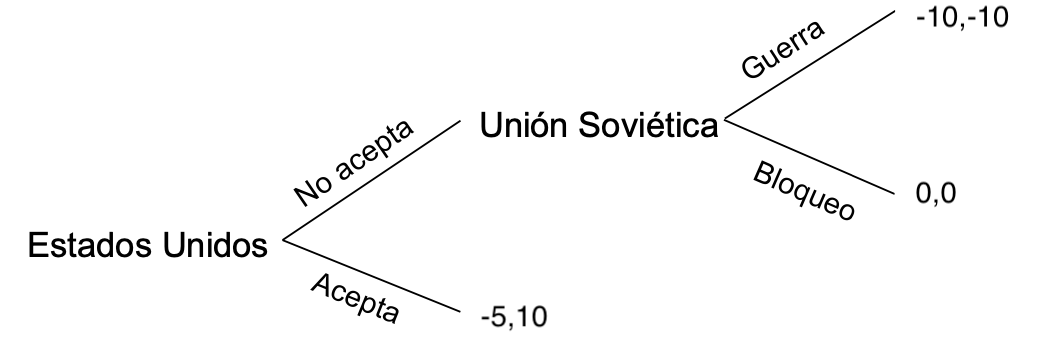
\includegraphics[scale=0.5]{Figuras/juegos secuencia.png}  
\end{center}
Las estrategias serán un plan de acción, en esta caso serían (Acepta, No Acepta y Guerra, No Acepta y Bloqueo).

Para resolver estos juegos uno tiene que seguir un método inductivo, resolver desde el futuro hacia el pasado. ¿Por qué resolver de adelante hacia atrás? Porque si resolvieramos como en juegos simultáneos no estaríamos contando si la amenaza (en este caso una respuesta bélica) es creíble. 

Si plantearamos de manera simultánea encontramos dos EN, uno (el de Acepta y Guerra) en que \textbf{no es secuencialmente racional}, para que ese equilibrio sea posible Estados Unidos tiene que aceptar, sin embargo veremos a continuación por qué si Estados Unidos no acepta la Unión Soviética nunca responderá con una respuesta bélica.

\begin{table}[!htbp]
    \centering
    \caption{Dominio sobre Berlín}
    \setlength{\extrarowheight}{2pt}
    \begin{tabular}{*{4}{c|}}
      \multicolumn{2}{c}{} & \multicolumn{2}{c}{Unión Soviética}\\\cline{3-4}
      \multicolumn{1}{c}{} &  & Guerra & Bloqueo \\\cline{2-4}
      \multirow{2}*{Estados Unidos}  & Acepta & $(\underbar{-5},\underbar{10})$ & $(-5,10)$ \\\cline{2-4}
      & No acepta & $(-10,-10)$ & $(\underbar{0},\underbar{0})$ \\\cline{2-4}
    \end{tabular}
  \end{table}

El juego tiene que ser \textbf{secuencialmente racional} por lo que resolvemos de adelante hacia atrás. El resultado será un equilibrio perfecto en subjuegos (EPS).

Por lo tanto primero se resuelve la decisión de la Unión Soviética, la cual debiese decidir bloquear, y luego evaluar que decidirá Estados Unidos, la cual debiese no aceptar. 

\begin{center}
    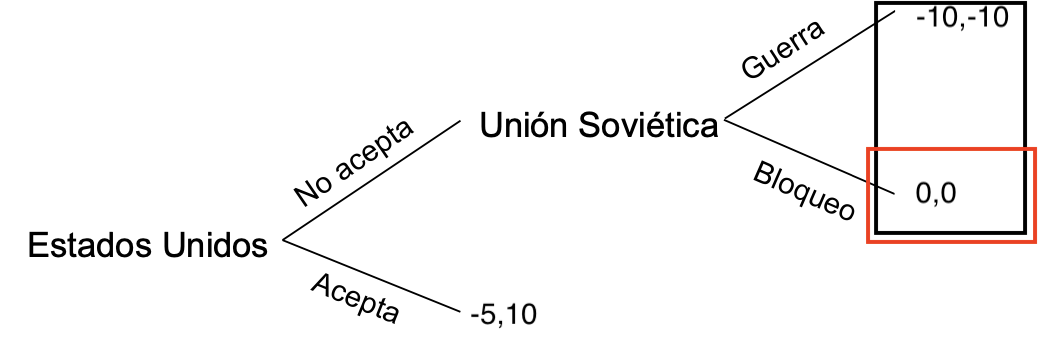
\includegraphics[scale = 0.50]{Figuras/Inducción.png}
\end{center}

\subsubsection*{Relación EN y EPS}

En un juegos secuencial puedes obtener EN que no sean coherentes con las amenazas creíbles. Los EPS siempre son coherentes con la credibilidad de las amenazas. \textbf{Un EN no siempre es un EPS, pero un EPS siempre es un EN}. 

\subsection{Estrategias Mixtas}